%%%%%%%%%%%%%%%%%%%%%%%%%%%%%%%%%%%%%%%%%%%%%%%%%%%%%%%%%%%%%%%%%%%%%%%%%%%%%%%%
%
% File: $Id$
%
% Change log at end.
%
% NOTE LACK OF DOCUMENT CLASS!
% This file must be \input into a "driver" file that sets the required
% beamer class options (notes, handout, etc.).
%
%%%%%%%%%%%%%%%%%%%%%%%%%%%%%%%%%%%%%%%%%%%%%%%%%%%%%%%%%%%%%%%%%%%%%%%%%%%%%%%%


\usepackage{beamerthemenzcs}
\usepackage{pgf,pgfarrows,pgfnodes}
\usepackage{graphicx}
\usepackage{calc}
\usepackage[absolute,overlay]{textpos}
\usepackage[normalem]{ulem}


% graphicx setup
\graphicspath{{images/}}


% hyperref setup
\hypersetup{colorlinks=false}


% textpos setup
\setlength{\TPHorizModule}{1cm}
\setlength{\TPVertModule}{1cm}


% document setup
\colorlet{dullgreen}{green!60!black}
\renewcommand{\ttdefault}{blg}

\footerleft{XML for Fun \& Profit}
\footercenter{August 26, 2004}
\footerright{\insertframenumber}

\author{Nigel Stanger}
\title{\textbf{XML for Fun and Profit}}
\institute{Department of Information Science, \\ University of Otago}
\date{August 26, 2004}


\begin{document}


%%%%%%%%%%%%%%%%%%%%%%%%%%%%%%%%%%%%%%%%%%%%%%%%%%%%%%%%%%%%%%%%%%%%%%%%%%%%%%%%


\frame
{
	\titlepage	

	\note{~}
}


%%%%%%%%%%%%%%%%%%%%%%%%%%%%%%%%%%%%%%%%%%%%%%%%%%%%%%%%%%%%%%%%%%%%%%%%%%%%%%%%


\frame
{
	\frametitle{Overview}
	
	\tableofcontents
	
	\note{~}
}


%%%%%%%%%%%%%%%%%%%%%%%%%%%%%%%%%%%%%%%%%%%%%%%%%%%%%%%%%%%%%%%%%%%%%%%%%%%%%%%%


\section{Historical context}


%%%%%%%%%%%%%%%%%%%%%%%%%%%%%%%%%%%%%%%%%%%%%%%%%%%%%%%%%%%%%%%%%%%%%%%%%%%%%%%%


\newlength{\yearposition}
\newcounter{yearvalue}

\newcommand{\timeline}[1]{%
	\begin{textblock}{10}(1.4,7.75)%
		\tiny%
		\setcounter{yearvalue}{#1-1960}%
		\setlength{\yearposition}{\value{yearvalue}cm/4}%
		\begin{pgfpicture}{0cm}{0cm}{10cm}{1cm}%
			\color{beamerstructure}%
			\pgfputat{\pgfpoint{\yearposition}{0.55cm}}{\pgfbox[right,bottom]{#1}}%
			\color{nzcslightorange!75!nzcsdarkorange}%
			\pgfsetlinewidth{0.5pt}%
			\pgfrect[fill]{\pgfxy(0,0)}{\pgfpoint{\yearposition}{0.5cm}}%
			\color{black}%
			\pgfrect[stroke]{\pgfxy(0,0)}{\pgfxy(10,0.5)}%
			\pgfxyline(0,0)(0,0.75)%
			\pgfxyline(2.5,0)(2.5,0.75)%
			\pgfxyline(5,0)(5,0.75)%
			\pgfxyline(7.5,0)(7.5,0.75)%
			\pgfxyline(10,0)(10,0.75)%
			\pgfputat{\pgfxy(0,1)}{\pgfbox[center,top]{1960}}%
			\pgfputat{\pgfxy(2.5,1)}{\pgfbox[center,top]{1970}}%
			\pgfputat{\pgfxy(5,1)}{\pgfbox[center,top]{1980}}%
			\pgfputat{\pgfxy(7.5,1)}{\pgfbox[center,top]{1990}}%
			\pgfputat{\pgfxy(10,1)}{\pgfbox[center,top]{2000}}%
		\end{pgfpicture}%
	\end{textblock}%
}


%%%%%%%%%%%%%%%%%%%%%%%%%%%%%%%%%%%%%%%%%%%%%%%%%%%%%%%%%%%%%%%%%%%%%%%%%%%%%%%%


\subsection*{GML \& SGML}


%%%%%%%%%%%%%%%%%%%%%%%%%%%%%%%%%%%%%%%%%%%%%%%%%%%%%%%%%%%%%%%%%%%%%%%%%%%%%%%%


\usebackgroundtemplate{\includegraphics{IBM-logo-BG}}

\frame[containsverbatim]
{
	\frametitle{The Generalised Markup Language (GML)}

	\begin{itemize}
	
		\item IBM
		
		\item First use of \verb|<tag>|\ldots\verb|</tag>|
		
		\note{These things are properly known as \emph{elements}.}
	
	\end{itemize}
	
	\timeline{1969}
}

\usebackgroundtemplate{}


%%%%%%%%%%%%%%%%%%%%%%%%%%%%%%%%%%%%%%%%%%%%%%%%%%%%%%%%%%%%%%%%%%%%%%%%%%%%%%%%


\frame
{
	\frametitle{Standard Generalised Markup Language (SGML)}

	\begin{itemize}
	
		\item Markup language for general documents
		
		\item Document \emph{types} (DTD)
		
		\note{Document type \emph{declaration}.}
		
		\item Complex to use and process
	
	\end{itemize}
	
	\timeline{1986}
	
	\note{~}
}


%%%%%%%%%%%%%%%%%%%%%%%%%%%%%%%%%%%%%%%%%%%%%%%%%%%%%%%%%%%%%%%%%%%%%%%%%%%%%%%%


\subsection*{Precursors to the web}


%%%%%%%%%%%%%%%%%%%%%%%%%%%%%%%%%%%%%%%%%%%%%%%%%%%%%%%%%%%%%%%%%%%%%%%%%%%%%%%%


% \frame<all:0>
% {
% 	\frametitle{File Transfer Protocol (FTP)}
% 
% 	\begin{itemize}
% 	
% 		\item Postel \& Reynolds
% 	
% 		\item Easy sharing of files and documents
% 		
% 		\item Remote login + file system metaphor
% 	
% 	\end{itemize}
% 	
% 	\timeline{1985}
% 	
% 	\note{~}
% }


%%%%%%%%%%%%%%%%%%%%%%%%%%%%%%%%%%%%%%%%%%%%%%%%%%%%%%%%%%%%%%%%%%%%%%%%%%%%%%%%


\usebackgroundtemplate{\includegraphics{gopher-BG}}

\frame
{
	\frametitle{Digging for information: Gopher}
	
	\begin{itemize}
	
		\item University of Minnesota
		
		\item Hierarchical menu structure for organising distributed
		documents
		
		\item Killed by licensing fees (1993) and relative inflexibility
		vs.\ web
	
	\end{itemize}

	\timeline{1991}
	
	\note{~}
}

\usebackgroundtemplate{}


%%%%%%%%%%%%%%%%%%%%%%%%%%%%%%%%%%%%%%%%%%%%%%%%%%%%%%%%%%%%%%%%%%%%%%%%%%%%%%%%


\frame
{
	\frametitle{Wide Area Information Server (WAIS)}
	
	\begin{itemize}
	
		\item Thinking Machines, Inc.
		
		\item Distributed text searching system
		
		\item Killed by bankruptcy (1995); more primitive than web
	
	\end{itemize}

	\timeline{1991}
	
	\note{~}
}


%%%%%%%%%%%%%%%%%%%%%%%%%%%%%%%%%%%%%%%%%%%%%%%%%%%%%%%%%%%%%%%%%%%%%%%%%%%%%%%%


\subsection*{The web \& HTML}


%%%%%%%%%%%%%%%%%%%%%%%%%%%%%%%%%%%%%%%%%%%%%%%%%%%%%%%%%%%%%%%%%%%%%%%%%%%%%%%%


\frame
{
	\frametitle{The World Wide Web (WWW)}
	
	\begin{itemize}
	
		\item Berners-Lee (1989)
		
		\item Networks of hyperlinked documents
		
		\note{cf.\ Vannevar Bush's \emph{Memex} (1945?).}
		
		\item Mosaic web browser (1993) \(\Rightarrow\) wide acceptance
		
		\item Documents constructed using \emph{HTML}
	
	\end{itemize}

	\timeline{1991}
}


%%%%%%%%%%%%%%%%%%%%%%%%%%%%%%%%%%%%%%%%%%%%%%%%%%%%%%%%%%%%%%%%%%%%%%%%%%%%%%%%


\frame
{
	\frametitle{Hypertext Markup Language (HTML)}
	
	\begin{itemize}
	
		\item An SGML document type for hypertext documents
		
		\item Separation of content and presentation
		
		\note{HTML was originally designed so that it was up to the web
		browser as to how a document would be displayed. The document
		author had little control over document appearance. In other
		words, HTML was originally designed as a semantic markup
		language rather than a presentation markup language. This has been lost
		over the years.}
		
		\item Fixed set of elements
	
	\end{itemize}

	\timeline{1991}
}


%%%%%%%%%%%%%%%%%%%%%%%%%%%%%%%%%%%%%%%%%%%%%%%%%%%%%%%%%%%%%%%%%%%%%%%%%%%%%%%%


\usebackgroundtemplate{\includegraphics{browser-icons-BG}}

\frame
{
	\frametitle{HTML falls in with the wrong crowd}
	
	\begin{itemize}
	
		\item Netscape vs.\ Microsoft
		
		\note[item]{Remember the \texttt{<blink>} tag?}
		
		\item ``Error recovery'' \(\Rightarrow\) inconsistent rendering
		
		\note[item]{Attempts by browser vendors to display as wide a
		range pages as possible (including syntactically incorrect ones)
		means that you never quite know how a particular page is going
		to appear in any given browser.}
		
		\item Confusion of meaning with presentation
		
		\note[item]{Primarily driven by designers who were used to
		precise control of document page layout and appearance.}
		
		\item Enhanced functionality requirements
		
		\note[item]{Examples: shopping carts \(\Rightarrow\) cookies;
		page layout \(\Rightarrow\) HTML tables; etc.}
	
	\end{itemize}

	\timeline{1994}
}

\usebackgroundtemplate{}


%%%%%%%%%%%%%%%%%%%%%%%%%%%%%%%%%%%%%%%%%%%%%%%%%%%%%%%%%%%%%%%%%%%%%%%%%%%%%%%%


\usebackgroundtemplate{\includegraphics{energizer-bunny-BG}}

\frame
{
	\frametitle{HTML runs out of steam}
	
	\textbf{Need for:}
	
	\begin{itemize}
	
		\item Dynamic web documents
		
		\note[item]{This includes both documents that are dynamically
		generated, and documents that change on the fly as they are
		manipulated (DHTML).}
		
		\item Complex client-side validation
		
		\note[item]{These days typically handled by JavaScript.}
		
		\item Database connectivity
		
		\item Data transport
		
		\item Flexible and extensible semantics
		
	\end{itemize}

	\timeline{1997}
}

\usebackgroundtemplate{}


%%%%%%%%%%%%%%%%%%%%%%%%%%%%%%%%%%%%%%%%%%%%%%%%%%%%%%%%%%%%%%%%%%%%%%%%%%%%%%%%


\subsection*{The rise of XML}


%%%%%%%%%%%%%%%%%%%%%%%%%%%%%%%%%%%%%%%%%%%%%%%%%%%%%%%%%%%%%%%%%%%%%%%%%%%%%%%%


\frame
{
	\frametitle{Extensible Markup Language (XML)}
	
	\begin{itemize}
	
		\item Effectively a simplified version of SGML
		
		\item User-definable elements \(\Rightarrow\) domain-specific
		markup languages
		
	\end{itemize}

	\timeline{1998}
	
	\note{~}
}


%%%%%%%%%%%%%%%%%%%%%%%%%%%%%%%%%%%%%%%%%%%%%%%%%%%%%%%%%%%%%%%%%%%%%%%%%%%%%%%%


\frame
{
	\frametitle{HTML is now an \uline{XML} document type}
	
	\begin{itemize}
	
		\item XHTML
		
		\item Web pages now also XML documents
		
		\note{Technically speaking, at least, and only if they conform
		to the XHTML spec.}
		
		\item Stricter syntax \(\Rightarrow\) consistent rendering
	
	\end{itemize}

	\timeline{2000}
}


%%%%%%%%%%%%%%%%%%%%%%%%%%%%%%%%%%%%%%%%%%%%%%%%%%%%%%%%%%%%%%%%%%%%%%%%%%%%%%%%


\section{XML 101: The basics}


%%%%%%%%%%%%%%%%%%%%%%%%%%%%%%%%%%%%%%%%%%%%%%%%%%%%%%%%%%%%%%%%%%%%%%%%%%%%%%%%


\subsection*{Introduction}


%%%%%%%%%%%%%%%%%%%%%%%%%%%%%%%%%%%%%%%%%%%%%%%%%%%%%%%%%%%%%%%%%%%%%%%%%%%%%%%%


\usebackgroundtemplate{\includegraphics{big-tick-BG}}

\frame
{
	\frametitle{What XML \uline{is}}
	
	\begin{itemize}
	
		\item ``SGML lite''
	
		\item Plain text (easy to manipulate)
		
		\item Free-form
		
		\item Extensible (define your own elements)
		
		\item Content-neutral markup
		
		\item Hierarchically structured
		
		\item Extremely verbose
		
		\note{In fact, deliberately verbose.}
	
	\end{itemize}
}

\usebackgroundtemplate{}


%%%%%%%%%%%%%%%%%%%%%%%%%%%%%%%%%%%%%%%%%%%%%%%%%%%%%%%%%%%%%%%%%%%%%%%%%%%%%%%%


\usebackgroundtemplate{\includegraphics{big-cross-BG}}

\frame
{
	\frametitle{What XML \uline{isn't}}
	
	\begin{itemize}
	
		\item A language (!)
		
		\note[item]{Not in the programming sense, at least. It's really
		more of a mechanism for specifying different varieties of
		markup. The same argument applies to the claim that XML is a
		file format.}
	
		\item A replacement for HTML
		
		\note[item]{Although this was the original intent, XML has
		developed into much more than this.}
		
		\item Intended for human consumption
		
		\note[item]{Being plain text, however, the temptation is there
		to make the markup human-readable. Handy for debugging, but
		technically unnecessary (and just makes things more verbose).}
		
		\item A database
		
		\item A silver bullet
	
	\end{itemize}
}

\usebackgroundtemplate{}


%%%%%%%%%%%%%%%%%%%%%%%%%%%%%%%%%%%%%%%%%%%%%%%%%%%%%%%%%%%%%%%%%%%%%%%%%%%%%%%%


\frame
{
	\frametitle{\uline{Lots} of standards}
	
	\begin{columns}
		\begin{column}{5.6cm}
			\includegraphics[height=6cm,keepaspectratio]{w3-shot}
		\end{column}
		
		\begin{column}{5cm}
			\begin{itemize}
			
				\item W3C have at least 32 different XML-related specs
				
				\item OASIS have over 40!
			
			\end{itemize}
		\end{column}
	\end{columns}
	
	\note{~}
}


%%%%%%%%%%%%%%%%%%%%%%%%%%%%%%%%%%%%%%%%%%%%%%%%%%%%%%%%%%%%%%%%%%%%%%%%%%%%%%%%


\frame
{
	\frametitle{\uline{Lots} of standards (a semi-random selection)}
	
	\begin{columns}
		\begin{column}{5cm}
			\begin{itemize}
			
				\item XML Schema
				
				\item XML Stylesheet Language
				
				\item MathML
				
				\item ChemML
				
				\item Scalable Vector Graphics
				
				\item SyncML
				
				\item ebXML (e-Business)
				
				\item LegalXML
				
				\item Tax XML
			
			\end{itemize}
		\end{column}

		\begin{column}{5cm}
			\begin{itemize}
			
				\item XHTML
				
				\item GeographyML
				
				\item XGMML (graphs)
				
				\item APXL (presentations)
				
				\item Water (programming)
				
				\item DocBook
				
				\item WSDL (web services)
				
				\item SAML (security)
				
				\item UBL (business docs)
			
			\end{itemize}
		\end{column}
	\end{columns}
	
	\note[item]{ebXML, LegalXML, DocBook and UBL are all managed by OASIS
	(Organisation for the Advancement of Structured Information
	Standards), an open XML standards organisation. Several of the
	others are managed by the World Wide Web Consortium. Also seen:
	e-government, emergency management, voice, accessibility, \ldots}
	
	\note[item]{ebXML is a collection of XML standards for electronic
	business. UBL provides a standard library of business documents
	(purchase orders, invoices, etc.).}
}


%%%%%%%%%%%%%%%%%%%%%%%%%%%%%%%%%%%%%%%%%%%%%%%%%%%%%%%%%%%%%%%%%%%%%%%%%%%%%%%%


\subsection*{Basic constructs}


%%%%%%%%%%%%%%%%%%%%%%%%%%%%%%%%%%%%%%%%%%%%%%%%%%%%%%%%%%%%%%%%%%%%%%%%%%%%%%%%


\frame[containsverbatim]
{
	\frametitle{A simple example}
	
	\footnotesize
	\begin{verbatim}
<?xml version="1.0"?>
<purchase-order ID="8892737451" date="2004-08-26">
  <supplier ID="12345">
    <name>The Dark Lord Sauron</name>
    <address>c/o Peter Jackson, Miramar</address>
  </supplier>
  <line-items>
    <item ID="RNG1111">
      <description>The One Ring</description>
      <quantity>1</quantity>
      <unit-price currency="NZD">12.95</unit-price>
    </item>
  </line-items>
</purchase-order>
	\end{verbatim}
	
	\note{~}
}


%%%%%%%%%%%%%%%%%%%%%%%%%%%%%%%%%%%%%%%%%%%%%%%%%%%%%%%%%%%%%%%%%%%%%%%%%%%%%%%%


\frame[containsverbatim]
{
	\frametitle{XML is based on elements}
	
	\begin{verbatim}
<name>Bilbo Baggins</name>

<address>Bag End, Hobbiton</address>

<phone/>

<credit-card>
  <type>VISA</type>
  <number>1234567890987654</number>
  <expires>05/05</expires>
</credit-card>
	\end{verbatim}
	
	\note[item]{Every XML document must have a single \emph{root}
	element (so in the previous slide, the root element was
	\texttt{purchase-order}).}

	\note[item]{Elements can be empty (as with \texttt{phone} above,
	presumably because it's inapplicable).}
	
	\note[item]{Elements must nest correctly \(\Rightarrow\)
	\emph{well-formed} XML.}
	
	\note[item]{Mention namespaces.}
}


%%%%%%%%%%%%%%%%%%%%%%%%%%%%%%%%%%%%%%%%%%%%%%%%%%%%%%%%%%%%%%%%%%%%%%%%%%%%%%%%


\frame[containsverbatim]
{
	\frametitle{XML elements can have attributes}
	
	\begin{verbatim}
<address location="home">25 Eglinton Road</address>

<address location="work">University of Otago</address>

<credit-card type="VISA" expires="05/05">
  1234567890987654
</credit-card>
	\end{verbatim}
	
	\note{Attributes are properties of an element. Sometimes it may not
	be clear whether something should be an attribute or a nested
	element. Some rules of thumb: internal use vs.\ intended for output,
	metadata vs.\ actual data. Context can also be important.}
}


%%%%%%%%%%%%%%%%%%%%%%%%%%%%%%%%%%%%%%%%%%%%%%%%%%%%%%%%%%%%%%%%%%%%%%%%%%%%%%%%


\subsection*{Structure}


%%%%%%%%%%%%%%%%%%%%%%%%%%%%%%%%%%%%%%%%%%%%%%%%%%%%%%%%%%%%%%%%%%%%%%%%%%%%%%%%


\frame
{
	\frametitle{Specifying XML elements}
	
	\begin{itemize}
	
		\item On the fly (standalone)
		
		\note{Fine for one-off or internal stuff, but not ideal if you
		want portability.}
		
		\item Using a Document Type Definition (DTD)
		
		\note{Similar but not quite identical to SGML DTDs. Define valid
		domain-specific elements and attributes and strict ordering
		(\emph{valid} XML). No data types as such, and hard to construct.}
		
		\item Using an XML schema
		
		\note{More your typical DDL with data types, collection types
		(including unordered collections), constraints, etc., etc.
		Actually an XML document type, so extremely verbose, but much
		more flexible and easier to create than than DTDs.}
	
	\end{itemize}
}


%%%%%%%%%%%%%%%%%%%%%%%%%%%%%%%%%%%%%%%%%%%%%%%%%%%%%%%%%%%%%%%%%%%%%%%%%%%%%%%%


\frame[containsverbatim]
{
	\frametitle{Interacting with XML documents: XPath}
	
	\begin{itemize}
	
		\item Any XML document can be represented as a tree
		
		\item Hierarchical document structure \(\Leftrightarrow\)
		hierarchical file system directory structure
		
		\item Specify paths within document from root:
		
		\verb|/courseapproval/personal/studentno|
		
		\verb|/courseapproval/paperlist/paper[points="6"]|
	
	\end{itemize}
	
	\note{~}
}


%%%%%%%%%%%%%%%%%%%%%%%%%%%%%%%%%%%%%%%%%%%%%%%%%%%%%%%%%%%%%%%%%%%%%%%%%%%%%%%%


\section{Advanced features}


%%%%%%%%%%%%%%%%%%%%%%%%%%%%%%%%%%%%%%%%%%%%%%%%%%%%%%%%%%%%%%%%%%%%%%%%%%%%%%%%


\subsection*{Querying}


%%%%%%%%%%%%%%%%%%%%%%%%%%%%%%%%%%%%%%%%%%%%%%%%%%%%%%%%%%%%%%%%%%%%%%%%%%%%%%%%


\usebackgroundtemplate{\includegraphics{query-BG}}

\frame
{
	\frametitle{Query languages for XML data}
	
	\begin{itemize}
	
		\item XQuery (W3C)
		
		\item XQL
		
		\item SiXDML
		
		\note[item]{XQuery is the ``official'' XML query language
		sanctioned by W3C.}
		
		\note[item]{XQL is a query language closely derived from XPath.}
		
		\note[item]{SiXDML = Simple XML Data Manipulation Language. Looks
		a bit like an XML-enabled SQL.}
	
	\end{itemize}
}

\usebackgroundtemplate{}


%%%%%%%%%%%%%%%%%%%%%%%%%%%%%%%%%%%%%%%%%%%%%%%%%%%%%%%%%%%%%%%%%%%%%%%%%%%%%%%%


\subsection*{Transforming}


%%%%%%%%%%%%%%%%%%%%%%%%%%%%%%%%%%%%%%%%%%%%%%%%%%%%%%%%%%%%%%%%%%%%%%%%%%%%%%%%


\frame
{
	\frametitle{XML data are frequently transformed}
	
	\textbf{To alter the structure of the data:}

	\begin{description}
	
		\item[XML \(\rightarrow\) XML:] to translate from one format to
		another, filter out unwanted material, etc.
		
	\end{description}

	\textbf{To provide human readability:}
	
	\begin{description}
	
		\item[XML \(\rightarrow\) HTML:] for presentation on the web.
		Often dynamically generated
		
		\item[XML \(\rightarrow\) text:] either plain text or other text
		format like PostScript, RTF, \LaTeX, tab-delimited, etc.
	
	\end{description}
	
	\note{We write many of our course documents in XML, then transform
	to HTML for web display, and \LaTeX\ \(\Rightarrow\) PDF for print.}
}


%%%%%%%%%%%%%%%%%%%%%%%%%%%%%%%%%%%%%%%%%%%%%%%%%%%%%%%%%%%%%%%%%%%%%%%%%%%%%%%%


\frame
{
	\frametitle{XSLT specifies XML transformations}
	
	\begin{itemize}
	
		\item XSL Transformations
		
		\item Yet another XML dialect
		
		\item Template-based transformation language:
		
		\note[item]{XSLT is a primarily non-procedural programming
		language, superficially somewhat similar to Prolog in concept
		(SNOBOL?). It isn't a general purpose programming language,
		however; it is a special-purpose language oriented toward
		transforming XML data.}
		
		\begin{itemize}
		
			\item XSL templates specify \emph{how} to transform XML
			elements
			
			\note[item]{XSLT programs are not executed in linear order
			like conventional procedural programs. Rather, patterns
			(specified by XPath expressions) are matched against an XML
			document in a hierarchical manner. The first template to
			match a particular pattern is executed.}
			
			\item XPath expressions specify \emph{which} XML elements to
			transform
		
		\end{itemize}
		
		\item[\(\Rightarrow\)] Separation of content \& presentation
		
	\end{itemize}
}


%%%%%%%%%%%%%%%%%%%%%%%%%%%%%%%%%%%%%%%%%%%%%%%%%%%%%%%%%%%%%%%%%%%%%%%%%%%%%%%%


\frame
{
	\frametitle{Typical XML/XSLT workflows}
	
	\begin{columns}
		\begin{column}{12cm}
			\begin{pgfpicture}{0cm}{0cm}{12cm}{6.25cm}
				\only<1>{\pgfputat{\pgfxy(6,3.125)}{\pgfbox[center,center]{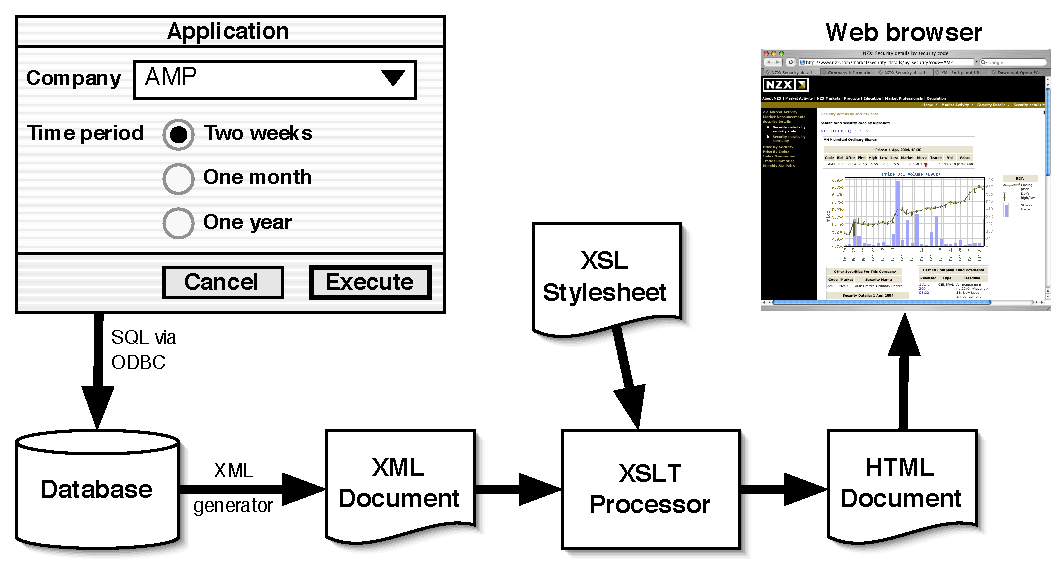
\includegraphics[width=12cm,keepaspectratio]{XML-Workflow-Web}}}}
				\only<2>{\pgfputat{\pgfxy(6,3.125)}{\pgfbox[center,center]{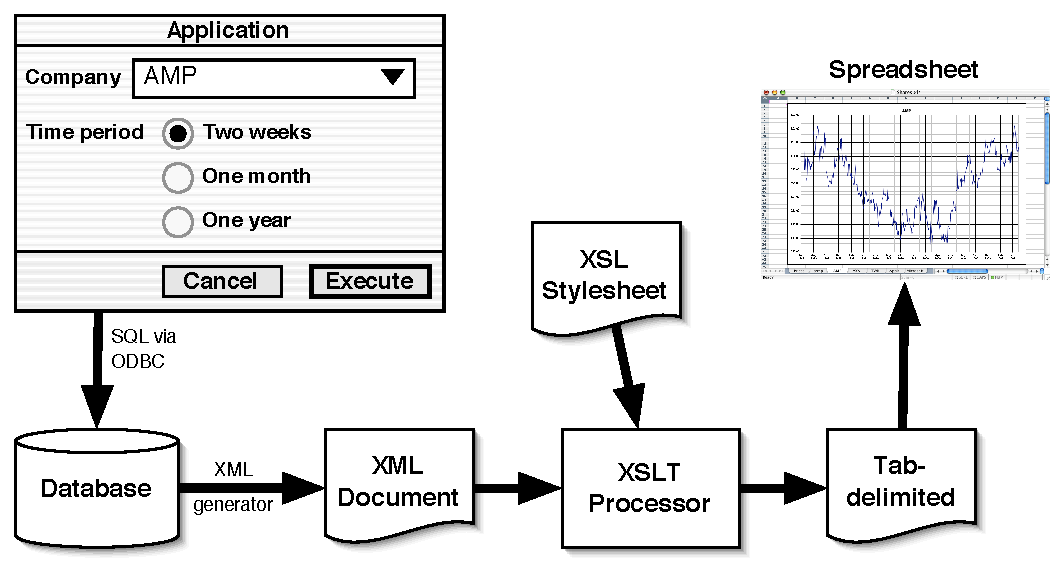
\includegraphics[width=12cm,keepaspectratio]{XML-Workflow-TSV}}}}
				\only<3>{\pgfputat{\pgfxy(6,3.125)}{\pgfbox[center,center]{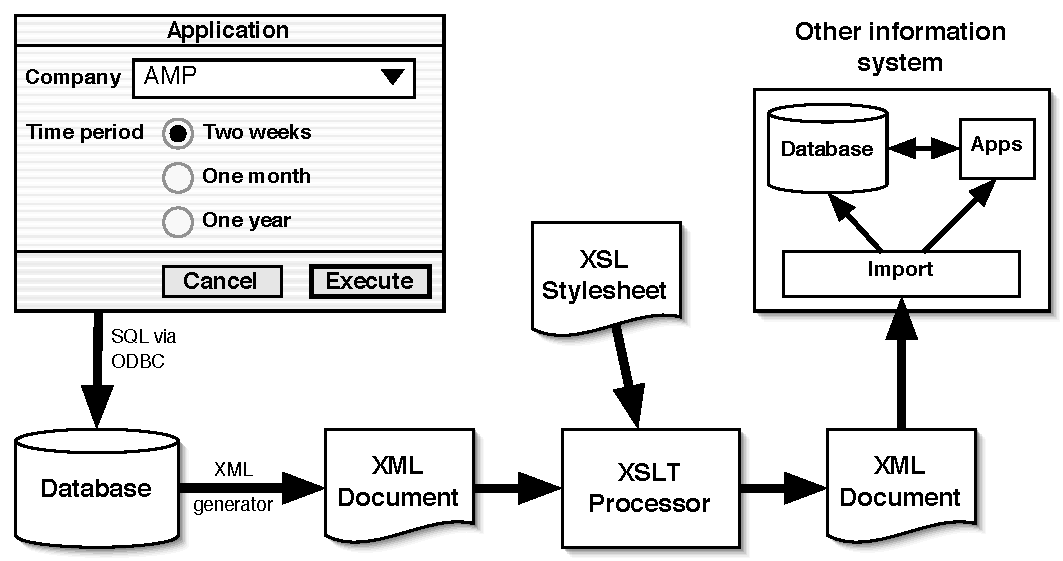
\includegraphics[width=12cm,keepaspectratio]{XML-Workflow-IS}}}}
			\end{pgfpicture}
		\end{column}
	\end{columns}
	
	\note<1>{The XML will often be generated from the database with the aid
	of an XML schema that describes how to map the original relational
	structures onto equivalent XML structures. Note that the generated
	XML will almost certainly be quite a different structure from the
	original (relationally-structured) data.}
}


%%%%%%%%%%%%%%%%%%%%%%%%%%%%%%%%%%%%%%%%%%%%%%%%%%%%%%%%%%%%%%%%%%%%%%%%%%%%%%%%


\section{Applications of XML}


%%%%%%%%%%%%%%%%%%%%%%%%%%%%%%%%%%%%%%%%%%%%%%%%%%%%%%%%%%%%%%%%%%%%%%%%%%%%%%%%


\frame
{
	\frametitle{What can be done with XML?}
	
	\begin{itemize}
	
		\item Domain specific markup languages (see earlier)

		\item Single-source dynamic document publication with multiple
		outputs
		
		\item Data interchange
		
		\note[item]{Basically anything that requires the storage and
		transport of structured data.}
		
		\item Metadata

		\item Aggregating data from multiple sources

		\item Data (document) storage and manipulation (i.e., database)
		
		\item Specification languages (e.g., for web services)
		
		\item[\alert{BUT:}] Strict hierarchical structure not suited to
		all applications

	\end{itemize}
	
	\note[item]{Note at this point that you're not 100\% familiar with
	everything that follows.}
}



%%%%%%%%%%%%%%%%%%%%%%%%%%%%%%%%%%%%%%%%%%%%%%%%%%%%%%%%%%%%%%%%%%%%%%%%%%%%%%%%


\subsection*{Single-source document publication}


%%%%%%%%%%%%%%%%%%%%%%%%%%%%%%%%%%%%%%%%%%%%%%%%%%%%%%%%%%%%%%%%%%%%%%%%%%%%%%%%


\frame
{
	\frametitle{XML can be used to publish documents}
	
	\centering
	
	\begin{columns}
	
		\begin{column}{12cm}
	
			\centering
			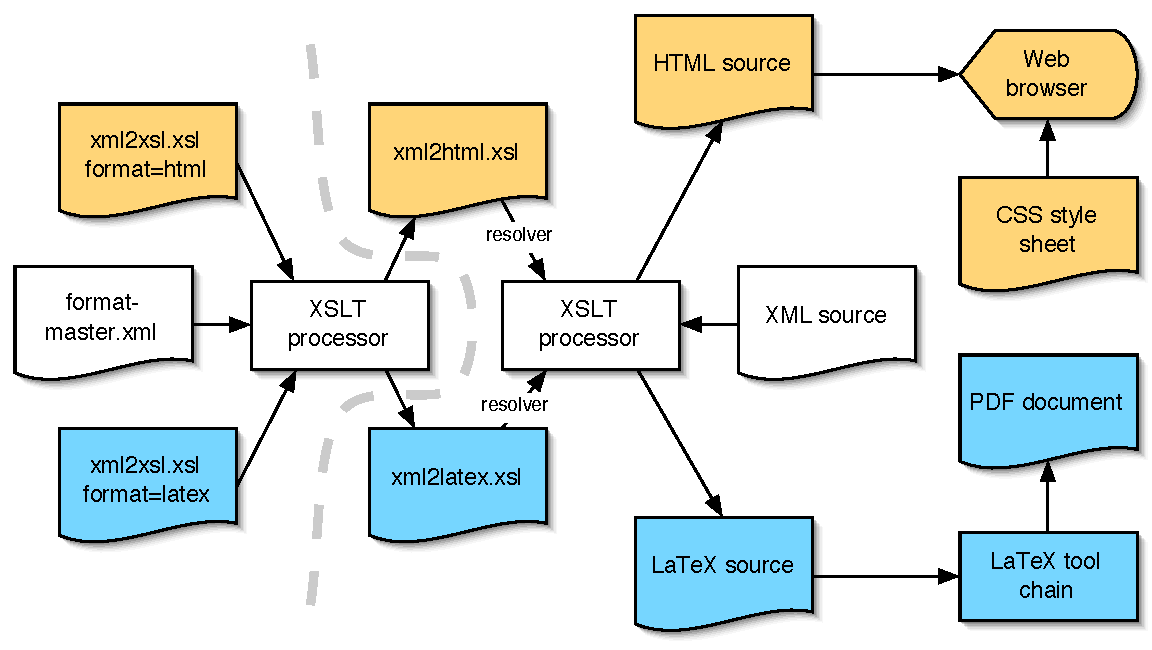
\includegraphics[height=6.5cm,keepaspectratio]{v2_workflow}
		
		\end{column}
		
	\end{columns}
	
	\note{Everything to the right of the thick dashed grey line is part
	of the day-to-day workflow. The stuff on the left on occurs when the
	master format is changed.}
}


%%%%%%%%%%%%%%%%%%%%%%%%%%%%%%%%%%%%%%%%%%%%%%%%%%%%%%%%%%%%%%%%%%%%%%%%%%%%%%%%


\subsection*{Data interchange}


%%%%%%%%%%%%%%%%%%%%%%%%%%%%%%%%%%%%%%%%%%%%%%%%%%%%%%%%%%%%%%%%%%%%%%%%%%%%%%%%


\frame
{
	\frametitle{XML can be used for data interchange}
	
	\begin{itemize}
	
		\item Export as XML \(\Rightarrow\) greater flexibility:

		\begin{itemize}
		
			\item Hard part is initial export

			\item Much easier to transform once in XML format
			
			\item Plain text never obsolete
		
		\end{itemize}
		
		\item XML wrappers for legacy systems
		
		\item XML namespaces for different industries, (e.g., ebXML)
		\(\Rightarrow\) standard interchange formats

	\end{itemize}
	
	\note{~}
}


%%%%%%%%%%%%%%%%%%%%%%%%%%%%%%%%%%%%%%%%%%%%%%%%%%%%%%%%%%%%%%%%%%%%%%%%%%%%%%%%


\subsection*{Metadata}


%%%%%%%%%%%%%%%%%%%%%%%%%%%%%%%%%%%%%%%%%%%%%%%%%%%%%%%%%%%%%%%%%%%%%%%%%%%%%%%%


\frame
{
	\only<2->{\usebackgroundtemplate{\includegraphics{nelson-BG}}}

	\frametitle{XML can be used to represent metadata}
	
	\begin{itemize}
	
		\item Resource Description Framework (RDF)

		\item \BoxHighlight<2>{Subject}-\BoxHighlight<3>{predicate}-\BoxHighlight<4>{object} expressions:
		
		``\BoxHighlight<2>{Nelson}'s \BoxHighlight<3>{postal code} is \BoxHighlight<4>{7001}''
		
		\item Attach to web pages to provide more meaning
		
		\item Easily machine-readable (e.g., search engines)

		\item Major component of \emph{Semantic Web}

	\end{itemize}
	
	\note<2>{~}
}

\usebackgroundtemplate{}


%%%%%%%%%%%%%%%%%%%%%%%%%%%%%%%%%%%%%%%%%%%%%%%%%%%%%%%%%%%%%%%%%%%%%%%%%%%%%%%%


\subsection*{Data aggregation}


%%%%%%%%%%%%%%%%%%%%%%%%%%%%%%%%%%%%%%%%%%%%%%%%%%%%%%%%%%%%%%%%%%%%%%%%%%%%%%%%


\frame
{
	\frametitle{XML can be used to aggregate data}
	
	\begin{itemize}
	
		\item Really Simple Syndication (RSS)
		
		\note[item]{More formally, RDF or Rich Site Summary.}

		\item Easily define data feeds (e.g., news articles)
		
		\note[item]{At present, RSS is mainly used to publish blog and
		news site updates in a format that is easily machine-readable.
		There is, however, no reason why this couldn't be applied to
		useful data. Example: automatically pulling updates to a
		supplier's catalogue off their web site and dumping them
		directly into your database (INFO 321 example).}
		
		\item \emph{Aggregator} pulls data from multiple feeds
		
		\note[item]{Thus, multiple supplier catalogues from multiple
		sites. The implicit assumption here is that the feeds are all
		for much the same thing, but a more sophisticated (probably
		custom) aggregator could integrate different kinds of data from
		various sources.}
		
		\item Incremental updates

	\end{itemize}
}


%%%%%%%%%%%%%%%%%%%%%%%%%%%%%%%%%%%%%%%%%%%%%%%%%%%%%%%%%%%%%%%%%%%%%%%%%%%%%%%%


\subsection*{Data storage}


%%%%%%%%%%%%%%%%%%%%%%%%%%%%%%%%%%%%%%%%%%%%%%%%%%%%%%%%%%%%%%%%%%%%%%%%%%%%%%%%


\frame
{
	\frametitle{XML can be used for data storage}
		
	\begin{itemize}
	
		\item Controversial
		
		\note[item]{\footnotesize Fabian Pascal argues fairly
		convincingly that XML databases are just a return to the
		hierarchical databases of old. XML is really better suited to
		storing \emph{document} structured data.}
		
		\item ``Structured'' vs.\ ``semi-structured'' vs.\
		``unstructured''
		
		\note[item]{\footnotesize These terms are rather badly misused.
		``Unstructured'', if interpreted literally, means ``random''.
		This is obviously not the case, however.}
		
		\item Relational: CLOB vs. ``shredding'' into relations
		
		\note[item]{\footnotesize Oracle provides XML support in the
		form of the XMLType data type, which is a specialised CLOB type.
		Shredding is usually only possible if there is an XML schema to
		describe the mapping; SQL Server provides native support for
		this. The ``big three'' all have similar XML support.}
		
		\item Non-relational: flat files vs.\ ``native'' XML database
		(eXist, Xindice, Tamino, \ldots)

		\item Document Object Model (DOM): XML-oriented API
		
		\note[item]{\footnotesize Note that the DOM is not a database
		API. It can just as easily be used to access plain XML documents
		(text files), and this is its most common use at present
		(Mozilla provides a DOM-based XML document browser in its
		sidebar). It is quite feasible however to provide a DOM wrapper
		to, say, a relational database, so that it looks like an XML
		data source to applications accessing it.}
	
	\end{itemize}
}


%%%%%%%%%%%%%%%%%%%%%%%%%%%%%%%%%%%%%%%%%%%%%%%%%%%%%%%%%%%%%%%%%%%%%%%%%%%%%%%%


\subsection*{Web services}


%%%%%%%%%%%%%%%%%%%%%%%%%%%%%%%%%%%%%%%%%%%%%%%%%%%%%%%%%%%%%%%%%%%%%%%%%%%%%%%%


\frame
{
	\only<2->{\usebackgroundtemplate{\includegraphics{haddock-BG}}}

	\frametitle{XML is the basis for web services}
		
	\begin{itemize}
	
		\item Web-accessible service providing programs
		
		\note<2>[item]{Examples: stock quotes, search engines,
		authentication (Microsoft Passport, credit cards), and my
		personal favourite, the Captain Haddock Insult Generator;
		basically anything that can be encapsulated in a chunk of code
		and called remotely. Really just XML-enabled RPC over HTTP.}
		
		\item Typically small
		
		\item A ``hot'' application of XML
		
		\item Sun (Java) vs.\ Microsoft (.NET)
		
		\note<2>[item]{Microsoft and Sun have clashed over standards for
		web services. Java and .NET web services are not guaranteed to
		be interoperable (different interpretations of data types,
		etc.). The WS-I (Web Services Interoperability) consortium is an
		attempt to resolve such problems.}
		
	\end{itemize}
}

\usebackgroundtemplate{}


%%%%%%%%%%%%%%%%%%%%%%%%%%%%%%%%%%%%%%%%%%%%%%%%%%%%%%%%%%%%%%%%%%%%%%%%%%%%%%%%


\frame
{
	\frametitle{A more technical definition}
		
	\begin{itemize}
	
		\item Remote procedure calls using XML and HTTP
		
		\item Transport protocol: HTTP
		
		\item Interaction protocols: \alert{XML-RPC}, \alert{SOAP},
		CORBA
		
		\item XML message format
		
		\item XML interface specification (WSDL)
		
	\end{itemize}
	
	\note{~}
}


%%%%%%%%%%%%%%%%%%%%%%%%%%%%%%%%%%%%%%%%%%%%%%%%%%%%%%%%%%%%%%%%%%%%%%%%%%%%%%%%


\frame
{
	\frametitle{Alphabet soup}
		
	\begin{description}
	
		\item[RPC] Remote Procedure Call (\(\Rightarrow\) XML-RPC)

		\item[SOAP] Simple Object Access Protocol

		\item[UDDI] Universal Description, Discovery and Integration
		(web service directory)

		\item[WSDL] Web Services Description Language

		\item[SAML] Security Assertion Markup Language

		\item[J2EE] Java 2 Enterprise Edition
		
	\end{description}
	
	\note{~}
}


%%%%%%%%%%%%%%%%%%%%%%%%%%%%%%%%%%%%%%%%%%%%%%%%%%%%%%%%%%%%%%%%%%%%%%%%%%%%%%%%


\usebackgroundtemplate{\includegraphics{web-services-BG}}

\frame
{
	\frametitle{Specific technology}
		
	\begin{description}
	
		\item[SOAP] for passing XML messages from one application to
		another, based on XML-RPC

		\item[WSDL] for specifying web service interfaces

		\item[Tools] Microsoft's .NET, J2EE (Java Beans), IBM's
		WebSphere, Oracle Application Server
		
		\note{Not suprisingly, a large number of web services are being
		implemented using .NET.}
		
	\end{description}
}

\usebackgroundtemplate{}


%%%%%%%%%%%%%%%%%%%%%%%%%%%%%%%%%%%%%%%%%%%%%%%%%%%%%%%%%%%%%%%%%%%%%%%%%%%%%%%%


\section{Conclusion}


%%%%%%%%%%%%%%%%%%%%%%%%%%%%%%%%%%%%%%%%%%%%%%%%%%%%%%%%%%%%%%%%%%%%%%%%%%%%%%%%


\frame
{
	\frametitle{Conclusion}
	
	\begin{itemize}
	
		\item XML specs \& tools now sufficiently mature
		
		\note{A problem with a lot of the tools was that the specs were
		still being developed, and were therefore something of a moving
		target. Things have now stabilised sufficiently for real work to
		be done, but the tools are still lagging behind the standards
		(but that is fairly typical).}
		
		\item XML reached critical mass about a year ago?
		
		\item Web services a ``hot technology''
			
	\end{itemize}
}


%%%%%%%%%%%%%%%%%%%%%%%%%%%%%%%%%%%%%%%%%%%%%%%%%%%%%%%%%%%%%%%%%%%%%%%%%%%%%%%%


\frame
{
	\frametitle{What's going to happen next?}
	
	\begin{itemize}
	
		\item Consolidation of existing specs and standards
		
		\item New versions of existing standards
		
		\note[item]{For example, a new version of XHTML that is a
		complete departure from XHTML 1.0, XSLT 2.0, etc.}
		
		\item Widespread adoption of interoperability standards such as
		ebXML
		
		\item Web services go mainstream
		
		\note[item]{It could be argued that web services already
		\emph{are} mainstream. We started teaching them this year.}
		
		\item New uses for XML keep emerging
		
		\note[item]{Water is one of the more unexpected uses of XML: an
		actual programming language using XML-like syntax!}
			
	\end{itemize}
}


%%%%%%%%%%%%%%%%%%%%%%%%%%%%%%%%%%%%%%%%%%%%%%%%%%%%%%%%%%%%%%%%%%%%%%%%%%%%%%%%


\frame
{
	\frametitle{Some useful sites}
	
	\textbf{XML-related standards}
		
	\begin{itemize}
	
		\item \url{<http://www.w3.org/>} (WWW Consortium)
		
		\item \url{<http://www.oasis-open.org/>} (OASIS)
		
		\item \url{<http://www.xml.org/>}
		
	\end{itemize}
	
	\textbf{Web services}
	
	\begin{itemize}
		
		\item \url{<http://www.webservices.org/>}
	
		\item \url{<http://www.ws-i.org/>} (interoperability)
		
		\item \url{<http://services.xmethods.net/>} (publicly available
		web services)
	
	\end{itemize}
	
	\note{~}
}


%%%%%%%%%%%%%%%%%%%%%%%%%%%%%%%%%%%%%%%%%%%%%%%%%%%%%%%%%%%%%%%%%%%%%%%%%%%%%%%%


\end{document}


%%%%%%%%%%%%%%%%%%%%%%%%%%%%%%%%%%%%%%%%%%%%%%%%%%%%%%%%%%%%%%%%%%%%%%%%%%%%%%%%
%
% $Log$
% Revision 1.9  2004/08/26 04:00:06  nstanger
% - Added XML->XML workflow diagram.
% - Added Captain Haddock image.
% - Added web service logos.
% - Tweaked a bunch of stuff.
% - Added web services slides.
% - Added conclusion slides.
% - Added more notes.
% - Modified XML example.
% - Added document publication workflow slide.
% - Delayed appearance of some backgrounds.
%
% Revision 1.8  2004/08/25 10:39:26  nstanger
% - Added hyperref setup to main document to fix colour of TOC entries.
% - Fixed vertical alignment of section entries in top banner.
%
% Revision 1.7  2004/08/25 05:17:52  nstanger
% - Shifted position of some background images.
% - Added yet more backgrounds!
% - Removed Intro section headings.
% - Tweaked several slides.
% - Added a bunch of notes.
% - Stole several slides from INFO 321.
% - Added XML workflow images.
% - Filled in content of XML basics and applications sections.
% - Deleted all the cruft from the old CIS seminar.
%
% Revision 1.6  2004/08/24 10:45:17  nstanger
% - Added some XML basics slides.
% - Finished off historical slides.
% - Switched off FTP slide.
% - Added more background images (big tick & cross).
%
% Revision 1.5  2004/08/24 06:26:19  nstanger
% - Added IBM logo background image.
%
% Revision 1.4  2004/08/24 04:44:51  nstanger
% - Added history slides.
%
% Revision 1.3  2004/08/23 10:45:19  nstanger
% - Added initial section headings.
% - Started adding content.
% - Added timeline drawing macro.
%
% Revision 1.2  2004/08/23 05:03:46  nstanger
% - Added makefile (still broken).
% - Tweaked source to use driver approach.
% - Added some images.
%
% Revision 1.1.1.1  2004/08/23 00:30:26  nstanger
% - Added XML presentation.
%
%%%%%%%%%%%%%%%%%%%%%%%%%%%%%%%%%%%%%%%%%%%%%%%%%%%%%%%%%%%%%%%%%%%%%%%%%%%%%%%%
